\documentclass[a4paper]{report}
\usepackage{amsmath,amsfonts,amssymb,latexsym}
\usepackage{graphicx,rotating,makeidx,xspace}
\usepackage{hyperref}
\usepackage[nottoc,notlot,notlof]{tocbibind}

\newcommand{\forget}[1]{}
\def \uppaal {{\sc Uppaal}}
\newcommand{\bang}{!}
\newcommand{\baror}{{\tt |}}
\sloppy

\def \fig#1 {\begin{figure}[htbp]\centering #1\end{figure}}
\def \tab#1 {\begin{table}[htbp]\centering #1\end{table}}
\def \mytab {\hbox{}\hspace{0.3cm}}
\def \beginlist#1 {
        \begin{#1}
        \setlength{\itemsep}{0pt}
        \setlength{\parskip}{0pt}
        \setlength{\topsep}{0pt}
        \setlength{\partopsep}{0pt}
        }

\def \cfunc#1#2#3#4 {\subsubsection{#2}
                     \index{C API!#2}
                     {\flushleft\em Synopsis: }{\tt #1 #2(#3);}
                     {\flushleft\em Description: }#4}

\def \cppfunc#1#2#3#4 {\subsubsection{#2}
                       \index{C++ API!#2}
                       {\flushleft\em Synopsis: }{\tt #1 #2(#3);}
                       {\flushleft\em Description: }#4}

\def \rclass#1 {\index{Ruby API!Class #1}}

\def \rfunc#1#2#3#4#5 {\subsubsection{#2}
		       \renewcommand{\bang}{"!}
		       \renewcommand{\baror}{{\tt "|}}
                       \index{Ruby API!Class #1!#2}
		       \renewcommand{\bang}{!}
		       \renewcommand{\baror}{{\tt |}}
                       {\flushleft\em Synopsis: }{\tt #2#3}
                       {\flushleft\em Description: }#4
                       {\flushleft\em Return: }#5}

\def \rtopfunc#1#2#3#4 {\subsubsection{#1}
                       \index{Ruby API!Module UDBM!#1}
                       {\flushleft\em Synopsis: }{\tt #1#2}
                       {\flushleft\em Description: }#3
                       {\flushleft\em Return: }#4}

\def \rconst#1#2 {\subsubsection{#1}
                  \index{Ruby API!Constants!UDBM::#1}
		  {\flushleft\em Description: }#2}

\def \example#1 {\newline Example:\\ {\tt #1}}

\makeindex

% Document begins here

\begin{document}
\setcounter{tocdepth}{4}
\renewcommand{\bibname}{References\label{REF}}

% Title

\title{{\uppaal} DBM Library 0.9\\Programmer's Reference}
\author{Alexandre David}
\maketitle
\newpage

% ToC

\tableofcontents
\newpage

% Manual :)

\chapter{Introduction}

Difference bound matrices (DBMs) are efficient data structures
commonly used in verification timed automata~\cite{ad94}. {\uppaal} is
a verification tool for timed automata and uses this library for
operating on DBMs. However, DBMs can only represent convex sets so the
library provides access to federations as well, an arbitrary union of
DBMs. The library architecture (Fig.~\ref{FIG:arch}) is as follows: A
core of C functions for basic operations on DBMs serves as a basis for
a C++ implementation of two main classes {\tt dbm\_t} and {\tt fed\_t}
that implement DBMs and federations. The C++ API is developper
friendly in the sense that memory allocation is hidden in the library
and these structures can be manipulated as simple scalar types cheaply
since the library implements reference counting and copy-on-write. A
Ruby binding is available to access federations with different
modules: {\tt udbm} is the core module for federations, {\tt udbm-gtk}
is the module for the graphical viewer (based on Gtk), {\tt udbm-sys}
is a higher level abstraction on system of constraints where DBMs are
entered only by means of constraints between clocks.

\fig{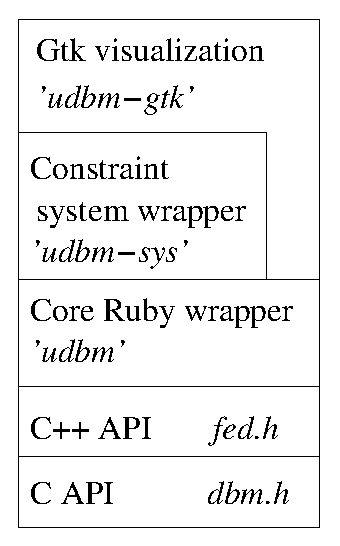
\includegraphics[width=0.35\linewidth]{architecture.eps}
\caption{Architecture of the DBM library.}
\label{FIG:arch}
}

\chapter{C API}

\section{Header file {\tt constraints.h}}
\label{SEC:Cconstraints}
\subsection{Types}
\index{C API!raw\_t}
\index{C++ API!raw\_t}
DBMs are matrices of clock constraints of the form $x_i-x_j<b_{ij}$ or
$x_i-x_j\le b_{ij}$. A clock constraint is internally encoded into the
type {\tt raw\_t}. In contrast bounds are integers ({\tt
int32\_t}).

\index{C API!constraint\_t}
The type {\tt constraint\_t} regroups the indices of
clock constraints and the encoded constraint itself (bound + strict or
non strict inequality). This type is also available with a constructor
in C++.
\begin{verbatim}
typedef struct {
    index_t i,j;
    raw_t value;
} constraint_t;
\end{verbatim}
%
Creation of constraints can be done with one of these two functions:
\index{C API!dbm\_constraint}
\index{C API!dbm\_constraint2}
\begin{verbatim}
constraint_t dbm_constraint(index_t i, index_t j,
                            int32_t bound, strictness_t strictness);

constraint_t dbm_constraint2(index_t i, index_t j,
                             int32_t bound, BOOL isStrict);
\end{verbatim}
The indices {\tt i} and {\tt j} correspond to the entry $(i,j)$ in the
DBM for the constraint. The bound is given followed by either a
strictness type (see Constants) or a boolean that says if the
constraint has a strict inequality or not.

\subsection{Constants}
\label{SUBSEC:Constants}
\index{C Constants!dbm\_INFINITY}
\index{C Constants!dbm\_OVERFLOW}
\index{C Constants!dbm\_LE\_ZERO}
\index{C Constants!dbm\_LS\_INFINITY}
\index{C Constants!dbm\_LS\_OVERFLOW}
\index{C Constants!dbm\_STRICT}
\index{C Constants!dbm\_WEAK}
\begin{tabular}{ll}
{\tt dbm\_INFINITY} & The infinity bound.\\
{\tt dbm\_OVERFLOW} & Bound to test for overflow.\\
{\tt dbm\_LE\_ZERO}  & Constraint encoding of $\le 0$.\\
{\tt dbm\_LS\_INFINITY} & Constraint encoding of $<\infty$.\\
{\tt dbm\_LS\_OVERFLOW} & Constraint to test for overflow.\\
{\tt dbm\_STRICT} & Enum type for strict inequalities ($<$).\\
{\tt dbm\_WEAK} & Enum type for weak inequalities ($\le$).\\
\end{tabular}

\subsection{Conversion Functions}
\cfunc{raw\_t}{dbm\_boundbool2raw}{int32\_t bound, BOOL isStrict}
{Convert a bound and a flag telling if the inequality is strict or not
to an encoded constraint.}

\cfunc{int32\_t}{dbm\_raw2bound}{raw\_t raw}
{Decode a constraint and return its bound.}

\cfunc{raw\_t}{dbm\_strictRaw}{raw\_t raw}
{Make a constraint strict (strict inequality).}

\cfunc{raw\_t}{dbm\_weakRaw}{raw\_t raw}
{Make a constraint weak (weak inequality).}

\cfunc{strictness\_t}{dbm\_raw2strict}{raw\_t raw}
{Decode a constraint and return its strictness (enum type, see the
constants in Subsection~\ref{SUBSEC:Constants}).}

\cfunc{BOOL}{dbm\_rawIsStrict}{raw\_t raw}
{Test if a constraint is strict -- return TRUE ($<$) or FALSE ($\le$).}

\cfunc{BOOL}{dbm\_rawIsWeak}{raw\_t raw}
{Test if a constraint is weak -- return TRUE ($\le$) or FALSE ($<$).}

\cfunc{strictness\_t}{dbm\_negStrict}{strictness\_t strictness}
{Negate the strictness of a constraint.}

\cfunc{raw\_t}{dbm\_negRaw}{raw\_t c}
{Negate a constraint, e.g., the negation of $<a$ is $\le -a$ and the
negation of $\le a$ is $< -a$.}

\cfunc{BOOL}{dbm\_isValidRaw}{raw\_t x}
{Test if a constraint is valie, i.e., it should not cause overflow in
(addition) operations.}

\cfunc{constraint\_t}{dbm\_negConstraint}{constraint\_t c}
{Negate a constraint and return its negation. The negation of
$x_i-x_j<b_{ij}$ is $x_j-x_i\le - b_{ij}$ and the negation of
$x_i-x_j\le b_{ij}$ is $x_j-x_i<-b_{ij}$.}

\cfunc{BOOL}{dbm\_areConstraintsEqual}{constraint\_t c1, constraint\_t
c2}{Test if two constraints c1 and c2 are equal, which is same indices
and same constraint value.}


\subsection{Addition of Constraints}

\cfunc{raw\_t}{dbm\_addRawRaw}{raw\_t x, raw\_t y}
{Addition of constraints. This is useful for the shortest path
computation. The constraints x or y may be infinity. Examples:
$(\le 2)+(\le 1)=(\le 3)$,
$(\le 2)+(<1)=(\le 3)$,
$(<2)+(<1)=(<3)$,
$(<=1)+(<\infty)=(<\infty)$.}

\cfunc{raw\_t}{dbm\_addRawFinite}{raw\_t x, raw\_t y}
{Addition of constraints with y being finite (not dbm\_LS\_INFINITY).}

\cfunc{raw\_t}{dbm\_addFiniteRaw}{raw\_t x, raw\_t y}
{Addition of constraints with x being finite (not dbm\_LS\_INFINITY).}

\cfunc{raw\_t}{dbm\_addFiniteFinite}{raw\_t x, raw\_t y}
{Addition of constraints with x and y being finite (not
dbm\_LS\_INFINITY).}

\cfunc{raw\_t}{dbm\_addFiniteWeak}{raw\_t x, raw\_t y}
{Specialized addition of constraints with x and y being finite (not
dbm\_LS\_INFINITY) and at least x or y being a weak constraint.}

\cfunc{raw\_t}{dbm\_rawInc}{raw\_t c, raw\_t i}
{Increment a constraint by i with a safe test for infinity. Notice
that the increment (i) is in raw\_t format. Addition of constraints
will result as $(\le 0)+(\le 0)=(\le 0)$, whereas increment
of constraints will result as $(\le 0) += 1 = (<1)$ with 1
corresponding to internal encoding of $(\le 0)$.}

\cfunc{raw\_t}{dbm\_rawDec}{raw\_t c, raw\_t d}
{Similarly to decrement a constraint. This has no effect if c is
infinity.}


\section{Header file {\tt dbm.h}}

A dbm is defined as a squared matrix of {\tt raw\_t}. The type {\tt raw\_t}
is the encoded clock constraint (see {\em constraints.h}).
IMPORTANT: In the system, you will typically have clocks
$x_1,x_2...,x_n$. The dbm has $x_0$ as the reference clock, hence
the dimension is equal to $n + 1$, which implies that we assume in all
the functions that the dimension is {\bf strictly} greater than 0.

The constraints of a DBM are refered as dbm[i,j] corresponding to the
element dbm[i*dim+j] of the {\tt raw\_t} array. As a reminder,
dbm[i,j] represents the constraint $x_i-x_j< b_{ij}$ or $x_i-x_j\le
b_{ij}$. The constraint encoding is described in {\em constraints.h}.

The C API does not support indirection table for clocks but the C++
API does. Dynamic mappings must be resolved before calling these
functions. Be careful when dealing with operation that
involve arrays of constraints (e.g., kExtrapolate).
As a common assumption for all operations on DBM:
$dim > 0$, which means at least the reference clock is
in the DBM.

A non empty DBM means the represented zone is non empty,
which is, for a closed dbm the diagonal elements are equal to 0.
As a common assumption, all the DBMs taken as arguments are closed
(the canonical form with the tightest constraints obtained by running
the shortest path algorithm) and non empty. Resulting DBMs are either
empty or closed and non empty.

The type {\tt cindex\_t} is used whenever an index or a dimension for a
DBM is expected. An index is between 0 and $2^{16}-1$ (even if the
representation is on 32 bits). Obviously since DBMs are square
matrices, this is a very reasonable limitation.


\subsection{Basic Functions}

\cfunc{void}{dbm\_init}{raw\_t *dbm, cindex\_t dim}
{Initialize a DBM {\tt dbm} of dimension {\tt dim} with $\le 0$ on the
diagonal and the first row, and infinity everywhere else, which is an
unconstrained DBM (with positive clocks).}

\cfunc{void}{dbm\_zero}{raw\_t *dbm, cindex\_t dim}
{Initialize a DBM {\tt dbm} of dimension {\tt dim} to the zero point
(origin), which is set all the constraints to $\le 0$.}

\cfunc{BOOL}{dbm\_isEqualToInit}{const raw\_t *dbm, cindex\_t dim}
{Test if the DBM {\tt dbm} of dimension {\tt dim} is equal to an
unconstrained DBM (as written by dbm\_init). Return TRUE if it is,
FALSE otherwise.}

\cfunc{BOOL}{dbm\_isEqualToZero}{const raw\_t *dbm, cindex\_t dim}
{Test if the DBM {\tt dbm} of dimension {\tt dim} is equal to the zero
point (as written by dbm\_zero). Return TRUE if it is, FALSE
otherwise.}

\cfunc{void}{dbm\_copy}{raw\_t *dst, const raw\_t *src, cindex\_t dim}
{Copy a DBM {\tt src} of dimension {\tt dim} to {\tt dst}. Notice that
the user has to make sure that {\tt dst} points to an array {\tt raw\_t[dim*dim]}.}

\cfunc{\\BOOL}{dbm\_areEqual}{const raw\_t *dbm1, const raw\_t *dbm2,
cindex\_t dim}
{Test if two DBMs are equal, i.e., are exactly identical, which makes
sense for DBMs in closed form. It is also possible to call {\tt
dbm\_relation} and test the result for {\tt base\_EQUAL} but this
function is better and implements an optimistic test, which means that
it will perform much better when DBMs are most often equal. This is
particularly desirable when using hash tables to store DBMs.}

\cfunc{uint32\_t}{dbm\_hash}{const raw\_t *dbm, cindex\_t dim}
{Compute a hash value for a DBM.}

\cfunc{\\BOOL}{dbm\_isPointIncluded}{const int32\_t *pt, const raw\_t
*dbm, cindex\_t dim}
{Test if a discrete point (i.e., clock valuation) is included in the
DBM (i.e., satisfies all the constraints of the DBM). Return TRUE if
it is the case, FALSE otherwise. Note that the dimension of the point
and the DBM must match. Also note that pt[0] should be 0 for this to
be meaningful unless the user wants to include an offset.}

\cfunc{\\BOOL}{dbm\_isRealPointIncluded}{const double *pt, const
raw\_t *dbm, cindex\_t dim}
{Test if a real point (at the precision of double, of course) is
included in the DBM. Return TRUE if it is the case, FALSE
otherwise. Note that the dimension of the point and the DBM must
match. Also note that pt[0] should be 0 for this to be meaningful
unless the user wants to include an offset.}

\cfunc{\\cindex\_t}{dbm\_shrinkExpand}{const raw\_t *dbmSrc, raw\_t
*dbmDst, cindex\_t dimSrc, const uint32\_t *bitSrc, const uint32\_t
*bitDst, size\_t bitSize, cindex\_t *table}
{Shrink and expand a DBM, which is, resize it and copy, add, or remove
clocks constraints corresponding to clocks that are copied, added, or
removed. The arguments are:
\begin{itemize}
\item {\tt dbmSrc}: The source DBM to resize. The necessary
constraints will be copied and the DBM will not be modified.
\item {\tt dbmDst}: The destination DBM (enough space must be
reserved) where to write the resulting DBM. It must be different from
{\tt dbmSrc}.
\item {\tt dimSrc}: The dimension of the source DBM. Note that the
dimension of the destination is not given in argument because it is
redundant with the information in {\tt bitDst}. Instead, it is
returned.
\item {\tt bitSrc} and {\tt bitDst}: Bit tables to mark which clocks
are represented in the source and the destination DBM. The idea is
that the user has a number of global clocks but the DBMs are
representing constraints on some of them only. The bit tables mark
which clocks are used in the DBMs, i.e., if bit $i$ is set then clock
$i$ is used. Of course clock $i$ is represented by some index $k$ in
the DBM and a translation table (or mapping) is computed and returned
as well. The first bit (bit 0) {\bf must} be set (it is the reference
clock). In addition, {\tt bitSrc} and {\tt bitDst} must be different
(have different bits), which is, the function is supposed to be called
if there is anything to do since it is slightly more expensive than a
simple copy (additional tests and computations are made).
\item {\tt bitSize}: The size of the bit table in integers (must be
$\le \lceil maxDim/32 \rceil$ where $maxDim$ is the maximal dimension,
or total number of clocks.
\item {\tt table}: Where to write the resulting translation table (or
mapping) for the result DBM.
\end{itemize}
The function returns the dimension of the resulting DBM (equal to the
number of bits set in {\tt bitDst}).}

\cfunc{\\void}{dbm\_updateDBM}{raw\_t *dbmDst, const raw\_t *dbmSrc,
cindex\_t dimDst, cindex\_t dimSrc, const cindex\_t *cols}
{Variant for resizing DBMs. Instead of giving arrays of bits, the user
provides an array of the clocks wanted in the destination DBM (with
the indices refering directly to the indices of the clocks of the
source DBM). The resulting DBM is written in {\tt dbmDst} (enough
space must be allocated), the original is read from {\tt dbmSrc}, the
dimensions of the destination and the source, are {\tt dimDst} and
{\tt dimSrc}. The table {\tt cols} which clock to take for the
destination and in which order: {\tt cols[i]} tells which clock from
the source to copy as clock $i$ in the destination and if the special
value {\tt ~0} is used then a new unconstrained clock is added. Only
the entries from 1 to dimDst-1 are meaningful with the entry at 0
being ignored since it corresponds to the reference clock that is
always present (must always be 0).}

\cfunc{void}{dbm\_swapClocks}{raw\_t *dbm, cindex\_t dim, cindex\_t x,
  cindex\_t y}
{Swap clocks {\tt x} and {\tt y}, which has the effect of swapping the
 corresponding constraints in the DBM {\tt dbm} of dimension {\tt dim}.}

\cfunc{BOOL}{dbm\_isDiagonalOK}{const raw\_t *dbm, cindex\_t dim}
{Test if the diagonal of a DBM is OK, which means that the constraints
are either less than $<0$ for an empty DBM or exactly $\le 0$ for a
non empty DBM. This is useful only for debugging. Return TRUE if the
diagonal is OK, FALSE otherwise.}

\cfunc{BOOL}{dbm\_isValid}{const raw\_t *dbm, cindex\_t dim}
{Return TRUE if a DBM is closed, not empty, and the constraints in the
first row are at most $\le 0$ (positive clocks), FALSE otherwise. It
is not necessary to test for the diagonal separately. This is a very
useful function to use in assertions, although it is expensive (cubic).}

\cfunc{const char*}{dbm\_relation2string}{relation\_t rel}
{Convert a relation\_t value to a meaningful string, which is useful
for user feedback.}

\cfunc{raw\_t}{dbm\_getMaxRange}{const raw\_t *dbm, cindex\_t dim}
{Compute the maximal range needed to store constraints of a DBM,
excluding infinity (a special large value). This function is useful if
the user intends to save DBMs on fewer than 32 bits.}


\subsection{DBM-DBM Operations}

\cfunc{\\void}{dbm\_convexUnion}{raw\_t *dbm1, const raw\_t *dbm2,
cindex\_t dim}
{Compute the convex union of two DBMs. This implements ``{\tt *dbm1 +=
*dbm2}'' where ``+'' refers to the convex union operator (used in the
C++ API).}

\cfunc{\\BOOL}{dbm\_intersection}{raw\_t *dbm1, const raw\_t *dbm2,
cindex\_t dim}
{Compute the intersection of two DBMs. This implements ``{\tt *dbm1 \&=
*dbm2}'' where ``\&'' refers to the intersection operator (used in the
C++ API). The function returns TRUE if the resulting DBM is not empty,
FALSE otherwise (and dbm1 is empty).}

\cfunc{\\BOOL}{dbm\_relaxedIntersection}{raw\_t *dbm1, const raw\_t
*dbm2, cindex\_t dim}
{Compute the intersection of two DBMs with their constraints
relaxed. A relaxed constraint is a constraint made non strict if it is
not infinity, e.g., $(<3)^+ = (\le 3)$. Infinity is always strict. The
result is stored in dbm1 and operation corresponds to ``{\tt *dbm1 =
(*dbm1)$^+$ \& (*dbm2)$^+$}''. The function returns TRUE if the
resulting DBM is not empty, FALSE otherwise (and dbm1 is empty).}

\cfunc{\\BOOL}{dbm\_haveIntersection}{const raw\_t *dbm1, const raw\_t
*dbm2, cindex\_t dim}
{Test if two DBM have a non empty intersection. The test is
approximate: The function returns FALSE	if the intersection is empty
for sure, or TRUE if the intersection is {\bf maybe} not empty.}


\subsection{Constraining Operations}

\cfunc{\\BOOL}{dbm\_constrain}{raw\_t *dbm, cindex\_t dim, cindex\_t i,
cindex\_t j, raw\_t constraint, uint32\_t *untouched}
{This is the only function in the API that returns DBMs {\bf that may
not be closed}. Calls to {\tt dbm\_isEmpty} may return erroneous results
unless dbm\_closex is called before. This function is useful in the
case where several constraints have to be applied on-the-fly to a DBM
without knowing in advance all of them. The DBM {\tt dbm} of dimension
{\tt dim} has its constraint $x_i-x_j$ constrained (or tightened
if possible) with the constraint {\tt constraint}. The function
returns FALSE if the DBM is empty for sure or TRUE if it is {\bf
maybe} not empty. The array {\tt untouched} is a bit array with {\tt
dim} bits, i.e., it is an array of $\lceil dim/32 \rceil$ {\tt
uint32\_t}. It must be initialized to 0 for the first call and then it
must not be modified between calls to dbm\_constrain. This array is
used to mark clocks that will be iterated over in the {\tt
dbm\_closex} function to reduce, if possible, the iterations (each
iteration is quadratic in function of dim).}

\cfunc{\\BOOL}{dbm\_constrainN}{raw\_t *dbm, cindex\_t dim, const
constraint\_t *constraints, size\_t n}
{Constrain the DBM {\tt dbm} of dimension {\tt dim} with {\tt n}
constraints. The resulting DBM is either closed and not empty (and the
function returns TRUE), or empty (and FALSE is returned). The
constraint of the DBM are tightened if the argument constraints are
tighter.}

\cfunc{\\BOOL}{dbm\_constrainIndexedN}{raw\_t *dbm, cindex\_t dim,
const cindex\_t *indexTable, const constraint\_t *constraints, size\_t
n}
{Constrain the DBM {\tt dbm} of dimension {\tt dim} with {\tt n}
constraints, {\bf but} constrain the constraints
$x_{indexTable[i]}-x_{indexTable[j]}$ instead of $x_i-x_j$ as the
previous function for all the constraints given in argument (a
constraint has indices $i$ and $j$, and a $value$ field encoding the
bound and the inequality). This function is useful in the case where
DBMs are dynamically resized and a global clock $x$ may not correspond
to the index $x$ of the DBM but to the index $indexTable[x]$.}

\cfunc{\\BOOL}{dbm\_constrain1}{raw\_t *dbm, cindex\_t dim, cindex\_t i,
cindex\_t j, raw\_t constraint}
{Constrain the DBM {\tt dbm} of dimension {\tt dim} with one
constraint given in argument (for the constraint $x_i-x_j$). Return
TRUE if the resulting DBM is not empty, FALSE otherwise.}

\cfunc{\\BOOL}{dbm\_constrainC}{raw\_t *dbm, cindex\_t dim,
constraint\_t c}
{This is a wrapper for {\tt dbm\_constrain1(dbm, dim, c.i, c.j,
c.value)}.}

\cfunc{\\BOOL}{dbm\_constrainClock}{raw\_t *dbm, cindex\_t dim,
cindex\_t x, int32\_t value}
{Apply the constraint $x == value$ for a clock {\tt x} to this
DBM. This is the same as applying $x-x_0 \le 0$ and $x_0-x \le 0$ to
the DBM, except that this call is more efficient than making two
consecutive calls. Return TRUE if the result is not empty, FALSE
otherwise.}


\subsection{Standard Operations}

\cfunc{void}{dbm\_up}{raw\_t *dbm, cindex\_t dim}
{Delay operation (future), also called strongest post-condition. The
function sets the constraints $(i,0)$ to infinity, i.e.,
$x_i-x_0<\infty$.}

\cfunc{void}{dbm\_down}{raw\_t *dbm, cindex\_t dim}
{Inverse delay operation (past), also called weakest
pre-condition. The function removes the lower bounds of the clocks and
update on-the-fly the closed form (some lower bounds may be induced by
diagonal constraints). The clocks are still positive.}

\cfunc{void}{dbm\_freeClock}{raw\_t *dbm, cindex\_t dim, cindex\_t k}
{Free a clock {\tt k}, which is, remove all the constraints of this
clock (except that the clock is still positive). This sets the
constraints $x_i-x_k<\infty$ and $x_k-x_i<\infty\;\forall i$) except
for $x_k-x_k\le 0$ and $x_0-x_k\le 0$.}

\cfunc{void}{dbm\_freeUp}{raw\_t *dbm, cindex\_t dim, cindex\_t k}
{Free the upper bounds of the clock {\tt k}, i.e., set the constraints
$x_k-x_i<\infty\;\forall i\neq k$).}

\cfunc{void}{dbm\_freeAllUp}{raw\_t *dbm, cindex\_t dim}
{Free the upper bounds for all the clocks (except the reference
clock), i.e., set all the constraints to $x_i-x_j<\infty$ for $i>0$
and $i\neq j$.}

\cfunc{BOOL}{dbm\_isFreedAllUp}{const raw\_t *dbm, cindex\_t dim}
{Test if calling {\tt dbm\_freeAllUp(dbm,dim)} has no effect on the
DBM, i.e., if all the clocks have their upper bounds freed: Return
TRUE if it is the case, FALSE otherwise.}

\cfunc{void}{dbm\_freeDown}{raw\_t *dbm, cindex\_t dim, cindex\_t k}
{Free the lower bounds of the clock {\tt k}, i.e., set the constraints
$(i,k)$ to $\le 0$ and tighten the DBM on-the-fly. In practice this
means to set $dbm[i,k] := dbm[i,0]\;\forall i \neq k$.}

\cfunc{void}{dbm\_freeAllDown}{raw\_t *dbm, cindex\_t dim}
{Free the lower bounds of all the clocks (except the reference clock),
i.e., set $dbm[i,k] := dbm[i,0]\;\forall i \neq k,\;\forall k>0$.}

\cfunc{BOOL}{dbm\_testFreeAllDown}{const raw\_t *dbm, cindex\_t dim}
{Test if calling {\tt dbm\_freeAllDown(dbm,dim)} has no effect on the
DBM, i.e., if all the clocks have their lower bounds freed: Return 0
if it is the case, or the value $(j << 16)|i$ where $(i,j)$
corresponds to the constraint from where the DBM differs from the
expected value.}

\cfunc{\\BOOL}{dbm\_satisfies}{const raw\_t *dbm, cindex\_t dim, cindex\_t
i, cindex\_t j, raw\_t constraint}
{Test if the DBM {\tt dbm} of dimension {\tt dim} satisfies the
constraint {\tt constraint} ($x_i-x_j<b_{ij}$ or $x_i-x_j\le b_{ij}$
encoded in {\tt constraint}). This corresponds to applying the
constraint to the DBM and checking if the result is not empty, except
that we do not apply the constraint. The function must not be
miss-used in testing consecutive constraints to conclude that the DBM
satisfies their conjuction, which is wrong. However, it is right for a
disjunction.}

\cfunc{BOOL}{dbm\_isEmpty}{const raw\_t *dbm, cindex\_t dim}
{Test if a DBM is empty (return TRUE) or not (return FALSE). An empty
DBM has a constraint stricly less than 0 (can be negative or can be
just $<0$), which results in no point satisfying the constraints. So
either there is such a constraint on the diagonal (and the DBM is
empty), or there is no such constraint but the DBM must be closed
(canonical form) for the result to be right. Generally all the
functions (except dbm\_constrain) maintain this invariant.}

\cfunc{BOOL}{dbm\_close}{raw\_t *dbm, cindex\_t dim}
{Apply the shortest path algorithm to the DBM to compute the tightest
possible constraints. This is the canonical form of the DBMs and we
refer to these DBM as being ``closed''. The result may be an empty
DBM, hence the return value: Return TRUE if the DBM is not empty,
FALSE otherwise. {\bf Note}: This algorithm is cubic in function of dim!}

\cfunc{BOOL}{dbm\_isClosed}{const raw\_t *dbm, cindex\_t dim}
{Test if this DBM is in its ``closed'' form. This function is only
useful for debugging or for assertions but be warned that it is as
expensive as {\tt dbm\_close} (in fact more expensive because there is
an internal allocation/copy/deallocation to test this). Return TRUE if
the DBM is closed, FALSE otherwise.}

\cfunc{\\BOOL}{dbm\_closex}{raw\_t *dbm, cindex\_t dim, const uint32\_t
*touched}
{This is a special version of {\tt dbm\_close} where only the clocks
marked in {\tt touched} will be tightened, i.e., if the bit $k$ is set
then the clock $k$ is tightened. This is useful to reduce the cost of
the close operation if we know that we need to tighten only certain
clocks, which is the case when constraining DBMs. Return TRUE if the
DBM is not empty, FALSE otherwise.}

\cfunc{BOOL}{dbm\_close1}{raw\_t *dbm, cindex\_t dim, cindex\_t k}
{Special version of {\tt dbm\_closex} for tightening only one clock
$k$. Return TRUE if the DBM is not empty, FALSE otherwise.}

\cfunc{\\BOOL}{dbm\_closeij}{raw\_t *dbm, cindex\_t dim, cindex\_t i,
cindex\_t j}
{Special and more efficient version of {\tt dbm\_closex} for
re-tightening a DBM after its constraint $x_i-x_j$ has been tightened!
Note that this works only for $x_i-x_j$ and its cost is $dim+dim^2$
instead of $2*dim^2$ if you call twice {\tt dbm\_close1} or if you
call {\tt dbm\_closex} with the two bits $i$ and $j$ set.}

\cfunc{\\void}{dbm\_tighten}{raw\_t *dbm, cindex\_t dim, cindex\_t i,
cindex\_t j, raw\_t c}
{This is a shortcut for {\tt dbm[i,j] := c} followed by a call to {\tt
dbm\_closeij(dbm, dim, i, j)}. The function {\bf assumes} that 1) it
is a tightening ($c < dbm[i,j]$) and 2) the tightening results in a non
empty DBM ($c+dbm[j,i] \ge 0$).}

\cfunc{BOOL}{dbm\_isUnbounded}{const raw\_t *dbm, cindex\_t dim}
{Test if a DBM is unbounded, i.e., if a point in the DBM can delay
indefinitely. Return TRUE if it is, FALSE otherwise.}

\cfunc{\\relation\_t}{dbm\_relation}{const raw\_t *dbm1, const raw\_t
*dbm2, cindex\_t dim}
{Compute the relation between two DBMs {\tt dbm1} and {\tt dbm2} of
dimension {\tt dim} in the sense of set inclusion. The return value
{\tt relation\_t} is an enumeration taking the values:
\begin{itemize}
\item {\tt base\_DIFFERENT} if dbm1 and dbm2 are not comparable,
\item {\tt base\_SUPERSET} if dbm1 is a strict superset of dbm2,
\item {\tt base\_SUBSET} if dbm1 is a strict subset of dbm2,
\item {\tt base\_EQUAL} if dbm1 is equal to dbm2.
\end{itemize}}

\cfunc{\\BOOL}{dbm\_isSubsetEq}{const raw\_t *dbm1, const raw\_t *dbm2,
cindex\_t dim}
{Test if dbm1 is a subset (non strict) of dbm2. Return TRUE if it is,
FALSE otherwise.}

\cfunc{\\BOOL}{dbm\_isSupersetEq}{const raw\_t *dbm1, const raw\_t
*dbm2, cindex\_t dim}
{Test if dbm1 is a superset (non strict) of dbm2. Return TRUE if it
is, FALSE otherwise.}


\subsection{Update Operations}

These operations correspond to updating a DBM to compute
operations at the clock level, e.g., {\tt x := 0} for
a reset of the clock x to 0, {\tt x := y} for copying the clock y to
x, etc \dots. Using a specialized version is more efficient than the
call to the general function {\tt dbm\_update}.

\cfunc{\\void}{dbm\_updateValue}{raw\_t *dim, cindex\_t dim, cindex\_t
x, int32\_t value}
{Update a clock {\tt x} to the value {\tt value}, i.e., compute
the operation {\tt x := value} where value is a positive integer.}

\cfunc{\\void}{dbm\_updateClock}{raw\_t *dbm, cindex\_t dim, cindex\_t x,
cindex\_t y}
{Update a clock {\tt x} to the clock {\tt y}, i.e., compute the
operation {\tt x := y}.}

\cfunc{\\void}{dbm\_updateIncrement}{raw\_t *dbm, cindex\_t dim, cindex\_t
x, int32\_t value}
{Increment a clock {\tt x} with {\tt value}, i.e., compute the
operation {\tt x := x + value}. The value may be negative but the user
has to make sure it is not too much negative, i.e., it will not result
in a negative value for the clock {\tt x}.}

\cfunc{\\void}{dbm\_update}{raw\_t *dbm, cindex\_t dim, cindex\_t x,
cindex\_t y, int32\_t value}
{This is a more general call to compute the operation {\tt x := y +
value}.}


\subsection{Relax Operations}

Relaxing constraints means to make them less or equal (a.k.a.\ weak)
when they are not $<\infty$. A constraint of the form $<b$ becomes
$\le b$. There are different relax operations to relax upper or lower
bounds. The point is that they recompute the closed form on-the-fly
whenever it is needed and the update is at most quadratic (and not
cubic if running {\tt dbm\_close}). However, it is important to note
that some functions may not be able to relax all the constraints they
are suppose to relax if they are induced by other tighter constraints
(a diagonal constraint may imply that another constraint must be
strict).

\cfunc{void}{dbm\_relaxUpClock}{raw\_t *dbm, cindex\_t dim, cindex\_t x}
{Relax the upper bounds of the clock {\tt x}, i.e., make the
constraints $x_k-x_i$ weak $\forall i$.}

\cfunc{void}{dbm\_relaxDownClock}{raw\_t *dbm, cindex\_t dim, cindex\_t x}
{Relax the lower bounds of the clock {\tt x}, i.e., make the
constraints $x_i-x_k$ weak $\forall i$.}

\cfunc{void}{dbm\_relaxAll}{raw\_t *dbm, cindex\_t dim}
{Relax all the constraints (those that are not $<\infty$ of course).}

\cfunc{void}{dbm\_relaxUp}{raw\_t *dbm, cindex\_t dim}
{Compute the smallest possible delay, which is the same as calling
{\tt dbm\_relaxDown(dbm, dim, 0)} for the reference clock!}

\cfunc{void}{dbm\_relaxDown}{raw\_t *dbm, cindex\_t dim}
{Compute the smallest possible inverse delay, which is the same as
calling {\tt dbm\_relaxUp(dbm, dim, 0)} for the reference clock!}


\subsection{Extrapolation Operations}\label{sec:dbmextra}

Extrapolations are approximation techniques to make sure that
exploration algorithms will terminate. Depending on the models (in
particular if diagonal constraints are used) the approximation can be
exact, or not. The following different extrapolation algorithms are
described in \cite{bbgp04} and the names correspond to the algorithms
of the paper. The arguments to the functions are the arrays of maximal
constants (possibly different lower and upper maximal bounds). It is
possible to give the special value {\tt -dbm\_INFINITY}, which has the
effect to ``free'' the corresponding clock, which is a trick for
implementing the so-called active clock reduction.

\cfunc{\\void}{dbm\_extrapolateMaxBounds}{raw\_t *dbm, cindex\_t dim,
const int32\_t *max}
{Classical extrapolation using maximal constants.}

\cfunc{\\void}{dbm\_diagonalExtrapolateMaxBounds}{raw\_t *dbm, cindex\_t
dim, const int32\_t *max}
{Diagonal extrapolation based on maximal bounds.}

\cfunc{\\void}{dbm\_extrapolateLUBounds}{raw\_t *dbm, cindex\_t dim,
const int32\_t *lower, const int32\_t *upper}
{Extrapolation based on lower and upper bounds.}

\cfunc{\\void}{dbm\_diagonalExtrapolateLUBounds}{raw\_t *dbm, cindex\_t
dim, const int32\_t *lower, const int32\_t *upper}
{Diagonal extrapolation based on lower and upper bounds.}


\section{Header file {\tt mingraph.h}}

DBMs can be represented more compactly by removing redundant
constraints and keeping only a minimal subset of
constraints~\cite{llpw:rtss97}. If we view DBMs as graphs we have
constraints, the edges, defined between clocks, the vertices. This
minimal representation is referred to as the {\em minimal graph}.
The API gives access to the minimal graph directly and provides means
of saving it somehow with different levels of compactness.

The idea is to have generic implementation that can be used with
standard allocation schemes (malloc, new) and with custom
allocators. This interface is in C to make it easy to wrap to other
languages so we use a generic function to allocate memory.  The
type of this function is 
{\tt int32\_t* function(uint32\_t size, void *data)}, where
{\tt size}e is the size in {\em int} to allocate, and it returns a
pointer to a {\tt int32\_t[size]}, and {\tt data} is other custom data.
Possible wrappers are:
\begin{itemize}
\item for a custom allocator Alloc\\
\begin{verbatim}
int32_t *alloc(uint32_t size, void *data) {
    return ((Alloc*)data)->alloc(size);
 }
\end{verbatim}
defined as {\tt base\_allocate} in {\em base/DataAllocator.h},
\item for malloc\\
\begin{verbatim}
int32_t *alloc(uint32_t size, void *) {
    return (int32_t*) malloc(size*sizeof(int32_t));
}
\end{verbatim}
defined as {\tt base\_malloc} in {\em base/c\_allocator.h},
\item for new\\
\begin{verbatim}
int32_t *alloc(uint32_t size, void *) {
    return new int32_t[size];
}
\end{verbatim}
defined as {\tt base\_new} in {\em base/DataAllocator.h}.
\end{itemize}
The allocator function and the custom data are packed
together inside the {\tt allocator\_t} type.

\cfunc{int32\_t*}{dbm\_writeToMinDBMWithOffset}
{const raw\_t *dbm, cindex\_t dim,\\
BOOL minimizeGraph, BOOL tryConstraints16,
alocator\_t c\_alloc, size\_t offset}
{Save a DBM in minimal representation.
The API supports allocation of larger data structures than needed
for the actual zone representation. When the {\tt offset} argument is
bigger than zero, {\tt offset} extra integers are allocated and the
zone is written with the given offset. Thus when {\em
int32\_t[data\_size]} is needed to represent the reduced zone, an
{\em int32\_t} array of size {\tt offset+data\_size} is allocated. The
first {\em offset} elements can be used by the caller. It is important
to notice that the other functions typically expect a pointer to
the actual zone data and not to the beginning of the allocated
block. Thus in the following piece of code, most functions expect
{\tt mg and not} memory:
\begin{verbatim}
int32_t *memory = dbm_writeToMinDBMWithOffset(...);
mingraph_t mg = &memory[offset]; 
\end{verbatim}

Notes:
If {\tt offset} is 0 and {\tt dim} is 1, NULL may be returned.
NULL is valid as an input to the other functions.
It could be possible to send as argument the maximal
value of the constraints that can be deduced from
the maximal constants but this would tie the algorithm
to the extrapolation.

The argument {\tt minimizeGraph} activates the minimal graph
reduction. The flag {\tt tryConstraints16} enables saving the
constraints on 16 bits (instead of 32). The allocation function
conforms to the previous specification of memory allocation.
}



%\section{Header file {\tt priced.h}}
%TODO

\section{Header file {\tt gen.h}}
%TODO

\section{Header file {\tt print.h}}
%TODO

%\section{Header file {\tt dbmfederation.h}}
% Deprecated


\chapter{C++ API}

\section{Header file {\tt constraints.h}}
\subsection{Type}
\index{C++ API!constraint\_t}
When compiling with g++ the structure {\tt constraint\_t} is available
with constructors.
\begin{verbatim}
struct constraint_t
{
    constraint_t() {}
    constraint_t(index_t ci, index_t cj, raw_t vij)
        : i(ci), j(cj), value(vij) {}

    index_t i,j;
    raw_t value;
};
\end{verbatim}

\subsection{Operator}

\cppfunc{bool}{operator {\tt <}}{const constraint\_t\& a, const
constraint\_t\& b}{Comparison of two constraints. An arbitrary
ordering has been chosen for sorting purposes. See {\tt constraint.h}
for the implementation.}

\section{Header file {\tt fed.h}}
\subsection{Extrapolation Operations}

To solve the untamable TA problem, UDBM supports the split extrapolation method described in \cite{bengtsson2003clock}.
For more information on extrapolation operations, see section \ref{sec:dbmextra}

\cfunc{\\void}{dbm::fed\_t::splitExtrapolate}{const constraint\_t *begin, const constraint\_t *end, const int32\_t *max}
{Split extrapolation based on maximal bounds.}

\section{Header file {\tt Valuation.h}}
%TODO

\section{Header file {\tt partition.h}}
%TODO

\section{Header file {\tt print.h}}
%TODO

\section{Header file {\tt inline\_fed.h}}
%TODO

\section{Header file {\tt Federation.h}}
%TODO


\chapter{Ruby Wrapper}

\section{Module {\tt udbm}}
The easiest way to use the module is to start with:\\
{\tt require 'udbm'\\
include UDBM\\}
to include the Ruby file udbm.rb and include the Ruby module UDBM that
is defined (similar to a namespace for accessing the classes). The
examples assume that ``include UDBM'' has been executed.

\rtopfunc{matrix}{}
{This is a shortcut for {\tt Matrix.new}.}
{a Matrix.}

\rtopfunc{Fed}{(dim)}
{This is the shortcut function to make writing federations more
natural. It expects a valid dimension as argument ($\ge 1$) and a
block that results in one Matrix or an array of matrices (or nil in
case of an empty federation). The trick is
to use the function {\tt matrix}.
\example{Fed(3) \# empty federation of dimension 3\\
Fed(4) \{\} \# empty federation of dimension 4 (variant)\\
Fed(2) \{ matrix <=0 <=-2 <=2 <=0 \} \# one DBM\\
Fed(2) \{[matrix <=0 <=-1 <=1 <=0,matrix <=0 <=-3 <=3 <=0 ]\} \# two}\\
However, constructing federations explicitly is not recommended since
it is not what is used in practice. The class methods {\tt zero} and
{\tt init} are here for this purpose.}
{a Fed.}

\subsection{Class UDBM::Constraint}
\rclass{UDBM::Constraint}

This class includes the module Comparable and has therefor access to
the methods declared in this module.
\rconst{INF}{The module defines the constant INF to access the bound infinity.}

\rfunc{UDBM::Constraint}{initialize}{(b, s = false)}
{This is the initialization method called by {\em new}. A constraint
is made of a bound and a strictness flag so the expected arguments are
the bound (b) and a boolean saying if the constraint is strict or not.
\example{Constraint.new(2,false)\\Constraint.new(1,true)}}
{The new instance (actually {\em new} returns it.).}

\rfunc{UDBM::Constraint}{bound}{}
{This is the attribute reader for the bound of the constraint.}
{The bound.}

\rfunc{UDBM::Constraint}{strict?}{}
{Test if the constraint is strict. This is in fact an attribute reader
for the strictness (boolean).}
{true if the constraint is strict, false otherwise.}

\rfunc{UDBM::Constraint}{bound{\tt =}}{(b)}
{Set the value of the bound of the constraint. The strictness is
changed if the argument is infinity (INF).}
{b.}

\rfunc{UDBM::Constraint}{strict{\tt =}}{(s)}
{Set the strictness of the constraint. A check is done in case the
bound is infinity (INF) to keep the constraint consistent. If the
constraint is infinity the strictness does not change.}
{s.}

\rfunc{UDBM::Constraint}{to\_s}{}
{String representation of a constraint.}
{a String.}

\rfunc{UDBM::Constraint}{raw}{}
{This gives access to the encoded value of constraints. Actually it
computes it on-the-fly since this class does not store an encoded
constraint but is only here as a helper class.}
{a numeric (Integer in principle).}

\rfunc{UDBM::Constraint}{{\tt <=>}}{(c)}
{Comparison function to make the constraint comparable. The ordering
corresponds to the ordering of the encoded value of constraints (raw),
which is consistent with the natural ordering of inequalities
($<0$,$\le 0$,$<1$,$\le1$,\dots).}
{-1, 0, or 1, as a standard {\tt <=>} method is supposed to do.}

\subsection{Class UDBM::Matrix}
\rclass{UDBM::Matrix}

This class is here only for convenience and testing. It is not
necessary for manipulating DBMs. A Matrix is simply a square matrix of
constraints and is used to construct DBMs manually or to get
constraints individually from DBMs.

\rfunc{UDBM::Matrix}{initialize}{(*a)}
{The initialization method expects constraints as arguments. No
argument will initialize an empty matrix.}
{self.}

\rfunc{UDBM::Matrix}{{\tt <}}{(b)}
{This operator is used as a trick to add constraints to the matrix. It
expects a bound as argument and the added constraint is $(<b)$.}
{self.}

\rfunc{UDBM::Matrix}{{\tt <=}}{(b)}
{This operator is used as a trick to add constraints to the matrix. It
expects a bound as argument and the added constraint is $(\le b)$.}
{self.}

\rfunc{UDBM::Matrix}{{\tt <<}}{(c)}
{This operator is similar to {\tt Array::<<} and adds constraints.}
{self.}

\rfunc{UDBM::Matrix}{dim}{}
{Compute the dimension corresponding to the current matrix.}
{$\lfloor\sqrt{size}\rfloor$.}

\rfunc{UDBM::Matrix}{size}{}
{Access to the number of element in the matrix.}
{a numeric (the size).}

\rfunc{UDBM::Matrix}{to\_s}{}
{String representation of a matrix.}
{a String.}

\rfunc{UDBM::Matrix}{inspect}{}
{Special formated string representation to be used in {\em irb}.}
{a String.}

\rfunc{UDBM::Matrix}{to\_a}{}
{Access to the internal array that stores the constraints. Notice that
if you do something like {\tt m.to\_a << Constraint.new(3,true)}, you
will add constraints to the matrix.}
{an Array.}

\rfunc{UDBM::Matrix}{[ ]}{(i,j)}
{Access the element of the matrix at $(i,j)$ (a constraint in principle).}
{Constraint expected.}

\rfunc{UDBM::Matrix}{set}{(i,j,c)}
{Set the constraint $(i,j)$ of in the matrix to be $c$.}
{self.}

\rfunc{UDBM::Matrix}{each}{\{ |x| \dots \}}
{Enumerate the constraints of the matrix.}
{self.}

\subsection{Class UDBM::Relation}
\rclass{UDBM::Relation}

The class Relation encapsulates the different constants representing
the possible results of a relation between DBMs (or in fact
federations here). When applying a relation from a federation on
another, e.g., {\tt a.relation(b)}, a Relation result is returned.

\rconst{Relation::Different}{Relation result when the two federations
are not comparable.}
\rconst{Relation::Subset}{Relation result when the federation 'a' is a
subset of 'b'.}
\rconst{Relation::Superset}{Relation result when the federation 'a' is
a superset of 'b'.}
\rconst{Relation::Equal}{Relation result when the federation 'a' is
equal to 'b'.}

\rfunc{UDBM::Relation}{{\tt ==}}{(r)}
{Test equality with another relation.}
{true or false.}

\rfunc{UDBM::Relation}{new}{(i)}
{It is possible to create relation instances on-the-fly. In this
case the argument is expected to be an integer between 0 and 3 to be
mapped to the proper constant.}
{self.}

\rfunc{UDBM::Relation}{to\_i}{}
{Convert a Relation to an Integer corresponding to the internal
numerical representation of relations.}
{a Fixnum.}

\rfunc{UDBM::Relation}{to\_s}{}
{Convert a Relation to its String representation.}
{a String.}

\rfunc{UDBM::Relation}{{\tt \&}}{(r)}
{Conjunction of relations.}
{a Relation.}

\rfunc{UDBM::Relation}{{\tt <=}}{(r)}
{``Weaker than'' comparison (or reverse implication). Note that
  ``Different'' really means ``not comparable''. Superset is weaker
  than equal but different is weaker than different only.}
{true or false.}

\subsection{Class UDBM::Fed}
\label{FED}
\rclass{UDBM::Fed}

The class Fed is a wrapper for the underlying C++ fed\_t class. There
is no support for individual DBMs from Ruby since it is only a
particular case of federations. If for some reason the clock
constraints need to be accessed, it is possible to get them via the
Matrix class.

\rfunc{UDBM::Fed}{new}{(*a)}
{The constructor takes a variable number of arguments. The different
ways to construct a federation are: (1) Constructor by copy, expects
one Fed; and (2) explicit DBMs, expects a list of Matrix instances
with the same dimension. There is a shortcut by using the function
Fed(dim) with a syntax that corresponds to the output of federations.}
{a Fed.}

\rfunc{UDBM::Fed}{Fed.zero}{(dim)}
{Create a federation with one DBM of dimension dim representing the
origin (the zero point).}
{a Fed.}

\rfunc{UDBM::Fed}{Fed.init}{(dim)}
{Create a federation with one DBM of dimension dim that is
unconstrained (infinity for all constraints except the lower bounds
set to 0 since clocks are positive).}
{a Fed.}

\rfunc{UDBM::Fed}{Fed.random}{(dim)}
{Create a random federation with a random number of DBMs, all of
dimension dim. This may be useful for testing.}
{a Fed.}

\rfunc{UDBM::Fed}{initialize}{(*a)}
{This is the initialization function called by {\tt new}. See {\tt new}.}
{a Fed (actually new returns it).}

\rfunc{UDBM::Fed}{to\_s}{}
{Standard method to get a String representation of the
federation. Notice that the output corresponds to the syntax of
declaring federations.}
{a String.}

\rfunc{UDBM::Fed}{to\_a}{}
{Convert a federation to an array of Matrix instances. This is the
method to use if you want to access individual constraints for some
reason.}
{an Array.}

\rfunc{UDBM::Fed}{size}{}
{Return the number of DBMs in the federation.}
{a Fixnum.}

\rfunc{UDBM::Fed}{dim}{}
{Return the dimension of all the DBMs of this federation. Notice that
all DBMs must have the same dimension.}
{a Fixnum.}

\rfunc{UDBM::Fed}{set\_dim\bang}{(dim)}
{Empty the federation and change its dimension to dim. As there is no
information on which clock constraints to keep, the only way to have a
consistent result is to have an empty federation.}
{self.}

\rfunc{UDBM::Fed}{copy}{}
{Return a copy of itself. Keep in mind that doing {\tt a = b} will
copy the reference of {\tt b} to {\tt a}, thus modifying {\tt a}
(e.g. {\tt a.up!}) will change {\tt b} as well. The copy method gives
a new reference.}
{a new Fed.}

\rfunc{UDBM::Fed}{empty?}{}
{Test if a federation is empty.}
{true if empty, false otherwise.}

\rfunc{UDBM::Fed}{unbounded?}{}
{Test if the federation is unbounded, i.e., if a point in the
federation can delay infinitely.}
{true if unbounded, false otherwise.}

\rfunc{UDBM::Fed}{empty\bang}{}
{Empty the federation.}
{self.}

\rfunc{UDBM::Fed}{intern\bang}{}
{Similarly to Java ``intern'' call on strings, this call will try to
share the DBMs internally so that all instances point to a unique data
structure whenever possible, thus saving memory. The user does not
have to worry if the federations are modified later, e.g., {\tt
a.intern! \dots a.up!}, the federations will be consistent and there
will be no undesirable side effect.}
{self.}

\rfunc{UDBM::Fed}{zero\bang}{}
{Set this federation to the zero point (the origin) with all the
clocks equal to zero.}
{self.}

\rfunc{UDBM::Fed}{init\bang}{}
{Remove all the constraints of this federation (except that all clocks
are always positive).}
{self.}

\rfunc{UDBM::Fed}{relation}{(f)}
{Compute a relation in the sense of set inclusion between this
federation and the argument federation. The result is typed as a
Relation class and is
\begin{itemize}
\item Relation::Superset if self is a strict superset of the argument
({\tt self > f}),
\item Relation::Subset if self is a strict subset of the argument
({\tt self < f}),
\item Relation::Equal if self is equal to the argument ({\tt self == f}), or
\item Relation::Different if self is not comparable to the argument.
\end{itemize}
}
{a Relation.}

\rfunc{UDBM::Fed}{convex\_hull}{}
{Compute the convex hull of all the DBMs in this federation.}
{a Fed.}

\rfunc{UDBM::Fed}{convex\_hull\bang}{}
{Set this federation to the convex hull of all its DBMs.}
{self.}

\rfunc{UDBM::Fed}{+}{(f)}
{Convex addition of this federation and another. The operator '+' is
for convex addition and the '|' for ordinary addition. The result is
the convex union of this federation and the argument (with this
federation being untouched).}
{a new Fed.}

\rfunc{UDBM::Fed}{convex\_add\bang}{(f)}
{Same a the '+' operator but modify this federation.}
{self.}

\rfunc{UDBM::Fed}{constrain\_clock\bang}{(clock,value)}
{Apply the constraint $clock==value$ for a given clock, which is
equivalent to applying both constraints $clock\le value$ and $clock
\ge value$ although it is shorter and faster to call this method.}
{self.}

\rfunc{UDBM::Fed}{constrain\bang}{(*args)}
{Apply a constraint of the form $x_i-x_j<b_{ij}$ or $x_i-x_j\le
b_{ij}$ to this federation. The expected arguments are either
$i,j,b,s$ for the indices $(i,j)$, the bound $b$ and a boolean $s$
telling if the bound is strict (true) or not (false), or $i,j,c$ for
the indices $(i,j)$ and a Constraint $c$.}
{self.}

\rfunc{UDBM::Fed}{{\tt \&}}{(f)}
{Compute the intersection of this federation and the argument
federation.}
{a new Fed.}

\rfunc{UDBM::Fed}{intersection\bang}{(f)}
{Set this federation to the intersection of itself and the argument
federation.}
{self.}

\rfunc{UDBM::Fed}{intersects?}{(f)}
{Test intersection between this federation and the argument
federation. The result is approximate and the ``no'' answer is
safe. To get an exact result (and more expensive to compute), you
should use {\tt !(a \& b).empty?} which would give the exact wanted
result.}
{true if there {\em may} be an intersection or false if there is no
intersection for sure.}

\rfunc{UDBM::Fed}{up}{}
{Compute the future. This is the delay, a.k.a.\ strongest
post-condition. In practice this operation removes the upper bounds on
the clock constraints.}
{a new Fed.}

\rfunc{UDBM::Fed}{up\bang}{}
{Apply the delay operation on this federation.}
{self.}

\rfunc{UDBM::Fed}{down}{}
{Compute the past. This is the ``reverse'' delay operation, a.k.a.\
weakest pre-condition. In practice this operation removes the lower
bounds while still maintaining the canonical form.}
{a new Fed.}

\rfunc{UDBM::Fed}{down\bang}{}
{Apply the past operation on this federation.}
{self.}

\rfunc{UDBM::Fed}{free\_clock}{(clock)}
{Free all the constraints for a given clock and return a new
federation.}
{a new Fed.}

\rfunc{UDBM::Fed}{free\_clock\bang}{(clock)}
{Same as free\_clock but modify this federation.}
{self.}

\rfunc{UDBM::Fed}{free\_up}{(clock)}
{Remove the upper bounds of a clock.}
{a new Fed.}

\rfunc{UDBM::Fed}{free\_up\bang}{(clock)}
{Same as free\_up but modify this federation.}
{self.}

\rfunc{UDBM::Fed}{free\_down}{(clock)}
{Remove the lower bounds of a clock.}
{a new Fed.}

\rfunc{UDBM::Fed}{free\_down\bang}{(clock)}
{Same as free\_down but modify this federation.}
{self.}

\rfunc{UDBM::Fed}{free\_all\_up}{}
{Remove all the upper bounds for all the clocks.}
{a new Fed.}

\rfunc{UDBM::Fed}{free\_all\_up\bang}{}
{Same as free\_all\_up but modify this federation.}
{self.}

\rfunc{UDBM::Fed}{free\_all\_down}{}
{Remove all the lower bounds for all the clocks.}
{a new Fed.}

\rfunc{UDBM::Fed}{free\_all\_down\bang}{}
{Same as free\_all\_down but modify this federation.}
{self.}

\rfunc{UDBM::Fed}{update\_value}{(x,value)}
{Apply the update {\tt x := value} for a given clock, where ``x'' is a
clock and ``value'' a positive integer.}
{a new Fed.}

\rfunc{UDBM::Fed}{update\_value\bang}{(x,value)}
{Same as update\_value but modify this federation.}
{self.}

\rfunc{UDBM::Fed}{update\_clock}{(x,y)}
{Apply the update {\tt x := y} for a given clock,
where ``x'' and ``y'' are clocks.}
{a new Fed.}

\rfunc{UDBM::Fed}{update\_clock\bang}{(x,y)}
{Same as update\_clock but modify this federation.}
{self.}

\rfunc{UDBM::Fed}{update\_increment}{(x,inc)}
{Apply the update {\tt x := x + inc} for a given clock, where ``x''
is a clock and ``inc'' is an integer. The user is responsible for
making sure that the increment is not too much negative since clocks
must stay positive.}
{a new Fed.}

\rfunc{UDBM::Fed}{update\_increment\bang}{(x,inc)}
{Same as update\_increment but modify this federation.}
{self.}

\rfunc{UDBM::Fed}{update}{(x,y,value)}
{Apply the update {\tt x := y + value} where ``x'' and ``y'' are
clocks and ``value'' is an integer. The user is responsible for making
sure that the result will give positive clock values.}
{a new Fed.}

\rfunc{UDBM::Fed}{update\bang}{(x,y,value)}
{Same as update but modify this federation.}
{self.}


\rfunc{UDBM::Fed}{satisfies?}{(*a)}
{Test if this federation satisfies a constraint of the form
$x_i-x_j<b_{ij}$ or $x_i-x_j\le b_{ij}$, i.e., if applying this
constraint to the federation results in a non empty federation. Notice
that it is fine to test for one constraint but testing several
constraints on a row is not correct because constraining a federation
with several constraint may yield an empty federation while
constraining it with the constraints separately may yield several non
empty federations. The arguments may be $(i,j,b,s)$ where $(i,j)$ are
the indices, $b$ the bound and $s$ a boolean telling if the constraint
is strict ($<$) or not ($\le$), or $(i,j,c)$ where $(i,j)$ are the
indices and $c$ a Constraint.}
{true if the federation satisfies the constraint, false otherwise.}

\rfunc{UDBM::Fed}{relax\_up}{}
{Make the upper bounds of all the clocks non strict. Notice that some
bounds may still be strict if they are inferred by strict diagonal
constraints. This method is equivalent to {\tt relax\_down\_clock(0)}.}
{a new Fed.}

\rfunc{UDBM::Fed}{relax\_up\bang}{}
{Same as relax\_up but modify this federation.}
{self.}

\rfunc{UDBM::Fed}{relax\_down}{}
{Make the lower bounds of all the clocks non strict. Notice that some
bounds may still be strict if they are inferred by strict diagonal
constraints. This method is equivalent to {\tt relax\_up\_clock(0)}.}
{a new Fed.}

\rfunc{UDBM::Fed}{relax\_down\bang}{}
{Same as relax\_down but modify this federation.}
{self.}

\rfunc{UDBM::Fed}{relax\_up\_clock}{(clock)}
{Make the upper bounds of a particular clock non strict. Some bounds
may still be strict if they are inferred by strict diagonal
constraints.}
{a new Fed.}

\rfunc{UDBM::Fed}{relax\_up\_clock\bang}{(clock)}
{Same as relax\_up\_clock but modify this federation.}
{self.}

\rfunc{UDBM::Fed}{relax\_down\_clock}{(clock)}
{Make the lower bounds of a particular clock non strict. Some bounds
may still be strict if they are inferred by strict diagonal
constraints.}
{a new Fed.}

\rfunc{UDBM::Fed}{relax\_down\_clock\bang}{(clock)}
{Same as relax\_down\_clock but modify this federation.}
{self.}

\rfunc{UDBM::Fed}{relax\_all}{}
{Make all the constraints non strict.}
{a new Fed.}

\rfunc{UDBM::Fed}{relax\_all\bang}{}
{Same as relax\_all but modify this federation.}
{self.}

\rfunc{UDBM::Fed}{subtraction\_empty?}{(fed)}
{Test if subtraction the argument federation to this federation (self
- fed) would give an empty federation, without computing the
subtraction itself if possible (internally). This federation is
untouched.}
{{\tt (self-fed).empty?}.}

\rfunc{UDBM::Fed}{\baror}{(fed)}
{Set union operator between this federation and the argument
federation.}
{a new Fed.}

\rfunc{UDBM::Fed}{union!}{(fed)}
{Same as the set union operator (|) but modify this federation.}
{self.}

\rfunc{UDBM::Fed}{{\tt -}}{(fed)}
{Subtraction operator between this federation and the argument
federation.}
{a new Fed.}

\rfunc{UDBM::Fed}{subtract\bang}{(fed)}
{Same as the subtraction operator but modify this federation.}
{self.}

\rfunc{UDBM::Fed}{merge\_reduce\bang}{}
{Apply a simple reduction algorithm on this federation to merge the
DBMs together if possible. The reduction tries to merge DBMs by pairs
and is able to remove included DBMs. The method computes a fixpoint
internally so there is no point in calling the method several times.}
{self.}

\rfunc{UDBM::Fed}{convex\_reduce\bang}{}
{Apply a more complex reduction based on convex union of several DBMs
chosen by some heuristic to merge them together if possible. This
method behaves at least as well as {\tt merge\_reduce} but is more
expensive.}
{self.}

\rfunc{UDBM::Fed}{partition\_reduce\bang}{}
{Partition the federation and run reduction algorithms on the
partitions. This method is more expensive but is as least as good as
{\tt convex\_reduce}.}
{self.}

\rfunc{UDBM::Fed}{expensive\_reduce\bang}{}
{Apply an expensive reduction algorithm based on subtractions to
eliminate included DBMs in the federation. Results may be very
different compared to the other reduction algorithms (although {\tt
partition\_reduce} is using it internally).}
{self.}

\rfunc{UDBM::Fed}{expensive\_convex\_reduce\bang}{}
{Recompute the federation, which is potentially very expensive but can
give very good results with respect to the number of DBMs.}
{self.}


{\bf\flushleft Important note.} All the reduce operations have
side-effects in the sense that if several federations refer to the
same internal structure, they will all be affected. The set is not
changed semantically but it may be simplified. In practice you may
notice it even with a copy (which might not update the graphical
viewer automatically if you are using it).

\rfunc{UDBM::Fed}{predt}{(bad)}
{Compute the predt operation described in \cite{cdfll05}. This
federation is considered to represent ``good'' states and the argument
is a set of ``bad'' states. The method computes the set of
predecessors of ``good'' avoiding the ``bad'' states, i.e., when
delaying from these states they will not intersect the ``bad'' states
and they will end-up in the ``good'' ones, if possible of course.}
{a new Fed.}

\rfunc{UDBM::Fed}{predt\bang}{(bad)}
{Same as predt but modify this federation.}
{self.}

\rfunc{UDBM::Fed}{remove\_included\_in}{(fed)}
{Compare the DBMs of this federation and the argument by pairs and
return a copy of this federation without the DBMs that are included in
those of the argument federation.}
{a new Fed.}

\rfunc{UDBM::Fed}{remove\_included\_in\bang}{(fed)}
{Same as remove\_included\_in but modify this federation and do not
copy anything.}
{self.}

\rfunc{UDBM::Fed}{{\tt <}}{(fed)}
{Set inclusion test: Test if this federation is strictly included in
the argument federation. The test involves more than testing DBMs by
pairs, it is a set inclusion test on the whole federation as a
set. This is equivalent to {\tt self.relation(fed) ==
Relation::Subset}, although possibly faster.}
{true if $self \subset fed$ (in the sense of set inclusion), false
otherwise.}

\rfunc{UDBM::Fed}{{\tt >}}{(fed)}
{Set inclusion test similar to {\tt <}: Test if this federation stricly
includes the argument federation. This is equivalent to {\tt
self.relation(fed) == Relation::Superset}, although possibly faster.}
{true if $fed \subset self$ (in the sense of set inclusion), false
otherwise.}

\rfunc{UDBM::Fed}{{\tt <=}}{(fed)}
{Set inclusion test similar to {\tt <}: Test if this federation is
included in or equal to the argument federation. This is equivalent to
{\tt self.relation(fed) == Relation::Subset || self.relation(fed) ==
Relation::Equal} that can be rewritten much more efficiently as {\tt
(self.relation(fed) \& Relation::Subset) != 0}, although possibly even
faster.}
{true if $self \subseteq fed$ (in the sense of set inclusion), false
otherwise.}

\rfunc{UDBM::Fed}{{\tt >=}}{(fed)}
{Set inclusion test similar to {\tt <}: Test if this federation includes
or is equal to the argument federation. This is equivalent to {\tt
self.relation(fed) == Relation::Superset || self.relation(fed) ==
Relation::Equal} that can be rewritten much more efficiently as {\tt
(self.relation(fed) \& Relation::Superset) != 0}, although possibly
even faster.}
{true if $fed \subseteq self$ (in the sense of set inclusion), false
otherwise.}
 
\rfunc{UDBM::Fed}{{\tt ==}}{(fed)}
{Set inclusion test similar to {\tt <}: Test if this federation is
equivalent to the argument federation. This is equivalent to {\tt
self.relation(fed) == Relation::Equal}, although possibley faster.}
{true if $self = fed$ (in the sense of set inclusion), false
otherwise.}

\rfunc{UDBM::Fed}{contains?}{(vec)}
{Test if this federation contains a clock valuation (a point in
dimension $n$ counting the reference clock 0). The argument (vec) is
either an array of integers or an array of floats giving the
coordinate of the point in dimension $n$ (and we have of course {\em
self.dim == n}). A clock valuation is included in a federation iff it
satisfies all the constraints of one of its DBMs.}
{true if the point is included in this federation, false otherwise.}

\rfunc{UDBM::Fed}{possible\_back\_delay}{(vec)}
{Compute the ``almost max'' possible delay backward from a point while
still staying inside the federation. It is 'almost max' since we want
a discrete value, which cannot me the max when we have strict
constraints. The precision is 0.5. 0.0 may be returned if the point is
too close to a border. The argument is expected to be an array of
floats giving the coordinate of the point in the federation.}
{a Float.}

\rfunc{UDBM::Fed}{min\_delay}{(point)}
{Compute the minimal delay to wait from a point to enter this
  federation. 0.0 is returned if the point is inside the
  federation. Infinity is returned if the point cannot enter this
  federation by delaying. A point is an array of floats giving the
  coordinate of a point. The dimension must match the dimension of the
  federation and the first coordinate (reference clock) is expected to
  be 0.0.
}

\rfunc{UDBM::Fed}{max\_back\_delay}{(point)}
{Compute the maximal delay to go back in time (back-delay or past) so
  that the (past-)point is still in this federation. If the point is
  or is not in the federation or the federation is not a connected set
  does not matter. 0.0 is returned if there is no such max delay or
  the max delay is already 0.0.}

\rfunc{UDBM::Fed}{delay}{(point)}
{Compute an interval delay where the first delay is given by {\tt
    min\_delay} and the second delay begin the minimum delay plus the
  time it is possible to wait and stay in the federation without
  leaving it {\em from} the point plus the minimum delay.} 

\rfunc{UDBM::Fed}{has\_zero?}{}
{Return True if this federation contains the zero point, false otherwise.}

{\flushleft\bf Extrapolation algorithms.} The following different
extrapolation algorithms are described in \cite{bbgp04} and the names
correspond to the algorithms of the paper. The arguments to the
methods are arrays of integers giving the constants but it is possible
to give the special value {\tt -INF}, which has the effect to ``free''
the corresponding clock, which is a trick for implementing active
clock reduction. The dimension of the array argument and the
federation should match.

\rfunc{UDBM::Fed}{extrapolate\_max\_bounds}{(vec)}
{Classical extrapolation using maximal constants.}
{a new Fed.}

\rfunc{UDBM::Fed}{extrapolate\_max\_bounds\bang}{(vec)}
{Same as extrapolate\_max\_bounds but modify this federation.}
{self.}

\rfunc{UDBM::Fed}{diagonal\_extrapolate\_max\_bounds}{(vec)}
{Diagonal extrapolation based on maximal bounds.}
{a new Fed.}

\rfunc{UDBM::Fed}{diagonal\_extrapolate\_max\_bounds\bang}{(vec)}
{Same as diagonal\_extrapolate\_max\_bounds but modify this
federation.}
{self.}

\rfunc{UDBM::Fed}{extrapolate\_lu\_bounds}{(low,up)}
{Extrapolation based on lower (low) and upper (up) bounds.}
{a new Fed.}

\rfunc{UDBM::Fed}{extrapolate\_lu\_bounds\bang}{(low,up)}
{Same as extrapolate\_lu\_bounds but modify this federation.}
{self.}

\rfunc{UDBM::Fed}{diagonal\_extrapolate\_lu\_bounds}{(low,up)}
{Diagonal extrapolation based on lower (low) and upper (up) bounds.}
{a new Fed.}

\rfunc{UDBM::Fed}{diagonal\_extrapolate\_lu\_bounds\bang}{(low,up)}
{Same as diagonal\_extrapolate\_lu\_bounds but modify this
federation.}
{self.}

\rfunc{UDBM::Fed}{drawing}{(border,width,height,x,y)}
{\label{DRAWFED}
Get drawing information for the drawing module (udbm-gtk). The
arguments are:
\begin{itemize}
\item border: the border to use (in pixels),
\item width: the width of the canvas for drawing (in pixels),
\item height: the height of the canvas for drawing (in pixels),
\item x,y: the clocks to use for the axis x and y.
\end{itemize}
Drawing is done in 2-D, which means that the federation is projected
on two given dimensions. The result is used internally by udbm-gtk.}
{an Array with the format [[ segments1 , polygon , segments2 , info ],\dots]
where every DBM gets a sub array. ``Segments1'' are segments for
border lines going to the axis x and y, ``polygon'' is a set of points
to draw a DBM, and ``segments2'' are additional segments for non
strict borders of the polygon. ``Info'' are tuples of the form
[x,y,value] to print a value at (x,y).}

\rfunc{UDBM::Fed}{point\_drawing}{(point,x,y)}
{Get drawing informatino for drawing a point for the drawing module
(udbm-gtk). This method must be called after {\tt drawing}. The
  arguments are the point (same dimension as the federation being
  displayed), and the clocks to choose for the projection on 2D. It
  returns an [[x1,y1,x2,y2],[x1,y1,x2,y2]] of the coordinates of two
segments for drawing a cross.}

\rfunc{UDBM::Fed}{formula}{(names)}
{Convert this federation to a readable formula (string of
characters). The argument is an Array of String to map clocks $j$ to
the names {\tt names[j-1]}. The clock reference (0) has no name and is
not part of the mapping.}
{a String.}

\rfunc{UDBM::Fed}{change\_clocks}{(clocks)}
{Change the clocks and resize the federation. The new federation has
its clock constraints coming from the original ones whenever
possible. The argument is an Array giving in order which clocks
(indices for the integers, without the clock reference) should be
present in the new federation, or {\tt nil} if a new clock is to be
inserted (then without constraints on it).}
{a new Fed.}

\rfunc{UDBM::Fed}{change\_clocks\bang}{(clocks)}
{Same as change\_clocks but modify this federation.}
{self.}

\rfunc{UDBM::Fed}{{\tt <<}}{(fed)}
{Operator similar to {\tt Array::<<} to compute a union of this federation
with the argument. This is equivalent to {\tt self.union!(fed)}.}
{self.}

\rfunc{UDBM::Fed}{dim{\tt =}}{(d)}
{Set a new dimension and empty the federation. This is equivalent to
{\tt self.set\_dim(d)} but returns d.}
{d.}

\section{Module {\tt udbm-callback}}

This short module is used by {\tt udbm-gtk} to detect changes on
federations to automatically update the graphical viewer. Normally
users do not need to use this module directly unless they wish to have
a change listener feature for federations. This module makes use of
Ruby ``magic''. The following methods are added in the class {\bf Fed}.

\rfunc{UDBM::Fed}{method\_added}{(id)}
{This method is automatically called whenever a method is defined in
Fed. The argument is the name of the method newly created. Of course,
it is preferrable to include the callback module before declaring
methods but there is a work-around to get rid of this limitation.}
{nil.}

\rfunc{UDBM::Fed}{register\_method}{(name)}
{This is the method that does the actual work of registering a method
for callback. Only the methods named ``something!'' are registered.}
{nil.}

\rfunc{UDBM::Fed}{add\_change\_listener}{(proc)}
{Add a change listener to call after any previously registered method
was executed. The argument is an object that provides a method {\tt
call(Fed,String)}, typically a Proc object with these two
arguments. When the listener is called, it is passed the instance of
Fed triggering the call and the name of the method invoked.}
{an Array of listeners.}

\section{Module {\tt udbm-sys}}

\subsection{Quick Start}
\label{QUICK}
Let's have a mini-tutorial to start. We use {\tt irb} for the
interactive Ruby interpreter. Start with including the modules:\\
\newline
{\tt prompt> irb\\
irb(main):001:0> require 'udbm-sys'\\
=> true\\
irb(main):002:0> require 'udbm-gtk'\\
=> true\\
irb(main):003:0> include UDBM\\
=> Object}\\
\newline
Declare a context for our clocks. The context is named ``C'' and {\tt c}
is our ruby reference to it. We can access our clocks as follows:\\
\newline
{\tt  irb(main):004:0> c=Context.create('C',:x,:y,:z)\\
=> \#<UDBM::Context\_C \{C.x,C.y,C.z\}>\\
irb(main):005:0> c.x\\
=> \#<UDBM::Context::Clock C.x>\\
irb(main):006:0> c.y\\
=> \#<UDBM::Context::Clock C.y>\\
irb(main):007:0> c.z\\
=> \#<UDBM::Context::Clock C.z>}\\
\newline
We can use a Ruby variable ``C'' to match the context name
(optional). Actually, names with capital letters are supposed to be
used for constants in Ruby. Let's also declare two sets referred to by
{\tt a} and {\tt b}.\\
\newline
{\tt irb(main):008:0> C=c\\
=> \#<UDBM::Context\_C {C.x,C.y,C.z}>\\
irb(main):009:0> a=(C.x>C.y) \& (C.z<4) \& (C.y<3)
=> \#<UDBM::Context\_C::Set\_C (((C.x>C.y) \& (C.z<4)) \& (C.y<3))>\\
irb(main):010:0> b=a \& ((C.x<2) | (C.x>=3))\\
=> \#<UDBM::Context\_C::Set\_C ((((C.x>C.y) \& (C.z<4)) \& (C.y<3)) \&
((C.x<2) | (C.x>=3)))>}\\
\newline
Please be careful with parenthesis to declare sub-expressions
otherwise the operator ``\&'' will be applied to clocks and we
want it to be applied to sets. These sets are defined naturally with
constraints on clocks as you can see. So far they are not evaluated
(internal representation, you don't have to worry about it). You can
see them with the following commands:\\
\newline
{\tt  irb(main):011:0> a.show('a')\\
=> \#<UDBM::Context\_C::Set\_C (C.y<3 \& C.y-C.x<0 \& C.z<4)>\\
irb(main):012:0> b.show('b')\\
=> \#<UDBM::Context\_C::Set\_C (3<=C.x \& C.y<3 \& C.z<4)|(C.x<2 \&
C.y-C.x<0 \& C.z<4)>}\\
\newline
Viewing is done by projecting the federation on two dimensions that
the user can choose. Notice that invoking the viewer triggers the
evaluation of the sets, which explains why they are now displayed
slightly differently. You can use most standard operations (see Fed in
Subsection~\ref{FED}) on sets, for example:\\
\newline
{\tt irb(main):012:0> b.up!\\
= > \#<UDBM::Context\_C::Set\_C (3<=C.x \& C.y-C.x<0 \& C.y-C.z<3 \&
C.z-C.x<1 \& C.z-C.y<4) | (C.x-C.y<2 \& C.x-C.z<2 \& C.y-C.x<0 \&
C.z-C.y<4)>}\\
\newline
The viewer is updated automatically thanks to the 'udbm-callback'
module (loaded automatically by 'udbm-gtk'). Update operations are
made extra user-friendly with operators defined on-the-fly:
\newline
{\tt irb(main):013:0> b.x=1\\
=> 1\\
irb(main):014:0> b.up!\\
=> \#<UDBM::Context\_C::Set\_C (1<=C.x \& C.x-C.y<=1 \& C.x-C.z<=1 \&
C.y-C.z<3 \& C.z-C.y<4) | (1<=C.x \& C.x-C.y<=1 \& C.x-C.z<=1 \&
C.y-C.z<2 \& C.z-C.y<4)>}\\
\newline
Access to clock {\tt x} in the set b is natural with {\tt b.x}. Notice
that the set keeps a reference to its context, you do not have to
worry about it. You can also change context to resize federations,
which we will describe later. The current federation of our example
can be simplified, which we can do with:\\
\newline
{\tt irb(main):014:0> b.reduce!\\
=> \#<UDBM::Context\_C::Set\_C (1<=C.x \& C.x-C.y<=1 \& C.x-C.z<=1 \&
C.y-C.z<3 \& C.z-C.y<4)>}\\
\newline
Now that we've seen the basic idea behind sets, let's examine how they
work.

\subsection{Class Fixnum}
\label{FIXNUM}

The standard class Fixnum has some methods added to make the
evaluation of formula easier, i.e., avoid to treat particular cases
and adopt Ruby philosophy of untyped objects that respond to
methods. These methods are used in evaluating expression of the form
{\tt x+c} or {\tt x-c} where ``x'' should refer to a clock (ID) and
``c'' should be a constant value (an offset).

\rfunc{Fixnum}{clock\_id}{}
{Return the clock ID associated with this object. Since this object is
not a clock, it is associated with the reference clock 0.}
{0.}

\rfunc{Fixnum}{offset}{}
{The offset associated with this object. Since this object is simply
an integer, the offset is itself.}
{self.}

\rfunc{Fixnum}{plus\_clock}{}
{This object is not a ``+''-expression.}
{nil.}

\rfunc{Fixnum}{minus\_clock}{}
{This object is not a ``-''-expression.}
{nil.}


\subsection{Class UDBM::Context}

When defining constraint systems, the user needs clocks. A set of
clocks is used to define federations and the size of the set
corresponds to the dimension of the federations. Clocks are therefor
defined within a ``context'' that groups these clocks to define
federations. A context is created with a name (for the context) and a
list of clocks (names too). A context is able to generate basic
federations (zero, init, random) and provides access to its clock
objects that are defined automatically (that's Ruby magic).

\rfunc{UDBM::Context}{name}{}
{The attribute reader for the name of a context.}
{a String.}

\rfunc{UDBM::Context}{clock\_names}{}
{The attribute reader for the names of the clocks of a context. The
names are prefixed by the name of the context.}
{an Array of String.}

\rfunc{UDBM::Context}{set\_class}{}
{The attribute reader for the class corresponding to the set of a
context. This is used within the module and users do not need
this. Classes are also objects, instances of the class {\tt Class}. In
Ruby everything is a class.}
{a Class.}

\rfunc{UDBM::Context}{context\_id}{}
{The attribute reader for the ID of a context. A context has an ID
based on the names of its clocks (used for changing context). The ID
is just another string constructed used internally. Users do not need
to worry about this method.}
{a Symbol.}

\rfunc{UDBM::Context}{short\_names}{}
{The attribute reader for the short names of the clocks of a
context. The difference with {\tt clock\_names} is that the names are
not prefixed (hence short). The returned type is different, though it
does not matter very much, it's for efficiency reasons when changing
context.}
{an Array of Symbol instances.}

\rfunc{UDBM::Context}{Context.create}{(name, *symbols)}
{Create a context with a given name and a list of
symbols (or strings) for the
clocks. \example{c=Context.create(``c'',:x,:y)}\\
A context has a unique name, which means you cannot declare different
contexts with the same name even if they have the same clocks.}
{a Context.}

\rfunc{UDBM::Context}{Context.get}{(name)}
{Get a previously defined context by its name. If the corresponding
context was not defined then the methods returns nil.}
{a Context or nil.}

\rfunc{UDBM::Context}{initialize}{(name, *symbols)}
{The initialization method of Context called by {\tt new}. Do not create
contexts directly with {\tt new}, use {\tt create} instead.}
{a Context (actually new returns it).}

\rfunc{UDBM::Context}{dim}{}
{The dimension of the federations that can be defined with
context. The dimension is equal to the number of clocks plus one (the
reference clock with the ID equal to 0, see~\ref{FIXNUM}).}
{a Fixnum.}

\rfunc{UDBM::Context}{zero}{}
{Create the federation representing the origin (point zero) within
this context, i.e., with the clocks defined in this context.}
{a Fed.}

\rfunc{UDBM::Context}{true}{}
{Create an unconstrained federation, i.e., corresponding to true in
terms of constraint (or the method {\tt init} on Fed), with the clocks
defined in this context.}
{a Fed.}

\rfunc{UDBM::Context}{false}{}
{Create an empty federation, i.e., corresponding to false in terms of
constraints, with the clocks defined in this context.}
{a Fed.}

\rfunc{UDBM::Context}{random}{}
{Create a random set, useful for testing only.}
{a Fed.}

\rfunc{UDBM::Context}{to\_s}{}
{The string representation of this context. This shows a list of
clocks.}
{a String.}

\rfunc{UDBM::Context}{update}{(context)}
{Compute the clock mapping from itself to the given context argument
for changing context (resizing of federations). The reference clock is
always mapped to 0 and is therefor not part of the mapping. The result
is an array of integers (IDs of the clocks) of the clocks of this
context (self) to be used in a given order for the target
context. Newly created clocks have {\tt nil} entries.
\example{a=Context.create("A",:x,:y)\\
=> \#<UDBM::Context\_A \{A.x,A.y\}>\\
b=Context.create("B",:y,:x,:z)\\
=> \#<UDBM::Context\_B \{B.y,B.x,B.z\}>\\
a.update(b)\\
=> [2, 1, nil]\\
b.update(a)\\
=> [2, 1]}\\
This method is used internally and may be used for other purposes.}
{an Array of Integer (or nil).}

\subsection{Class UDBM::Context::Clock}

The most useful features of clocks are their operators that allow
users to write formulas naturally to define constraints. The other
methods are useful internally to evaluate formulas to federations.

\rfunc{UDBM::Context::Clock}{context}{}
{The attribute reader for the context of this clock.}
{a Context.}

\rfunc{UDBM::Context::Clock}{initialize}{(context, index)}
{The initialization method to be called by {\tt new}. Users are not
supposed to define clocks directly but to access them from a context.}
{a Clock (actually {\tt new} returns it).}

\rfunc{UDBM::Context::Clock}{to\_s}{}
{String representation of this clock, i.e., its name prefixed by the
context name.}
{a String.}

\rfunc{UDBM::Context::Clock}{clock\_id}{}
{The clock ID of this clock, which corresponds to its index in
federations (of this clock's context) to access it.}
{a Fixnum.}

\rfunc{UDBM::Context::Clock}{offset}{}
{The offset of this object. Since this is a clock, its offset is
0. Integers have offsets equal to themselves. This is used internally
for evaluating formulas.}
{a Fixnum.}

\rfunc{UDBM::Context::Clock}{plus\_clock}{}
{The ``+ clock'' expression of this formula, which is itself for a
simple clock. Actually, the method returns the ID of this clock.}
{a Fixnum.}

\rfunc{UDBM::Context::Clock}{minus\_clock}{}
{The ``- clock'' expression of this formula, which is nothing for a
simple clock so the method returns nil.}
{nil.}

\subsubsection{Operators On Clocks}
\def \clockop#1 {\index{Ruby API!Class UDBM::Context::Clock!#1}#1\xspace}
Clocks have operators in order to write formulas of clock constraints
to describe sets. The operators that return sets (Context::Set\_XX
with XX being the name of the context) are: \clockop{{\tt ==}},
\clockop{{\tt <}},
\clockop{{\tt <=}},
\clockop{{\tt >}},
and
\clockop{{\tt >=}}. The operators that return sub-formulas
(Context::Formula) are
\clockop{{\tt +}}
and
\clockop{{\tt -}}. Notice that the class Formula has the same operators to
write formulas.


\subsection{Class UDBM::Context::Set}

The class Set represents sets of clock valuations. This class is not
supposed to be created directly by users. Instead, the Context class
will create the proper Set\_XX class on-demand where XX is the name of
the context. Only sets with the same context are compatible. For the
sake of simplicity we refer only to Set from now on. Sets are
represented internally as formulas (class Formula) or federations
(class SymbolicSet that wraps Federation). The convertion is
transparent for the user. Sets implement lazy evaluation of formulas,
which means that they are evaluated only when needed.

\rfunc{UDBM::Context::Set}{instance}{}
{Attribute reader for the actual representation of the set (formula or
federation). There is also a corresponding attribute writer that
should disappear one day.}
{a Formula or a SymbolicSet.}

\rfunc{UDBM::Context::Set}{initialize}{(instance)}
{The initialization method called by new. Users do not instantiate
sets directly. This is used by Context. The instance is either a
Formula or a SymbolicSet that are owned by this Set instance.}
{a Set (actually {\tt new} returns it).}

\rfunc{UDBM::Context::Set}{fed}{}
{Compute (if needed) the corresponding federation and return it. Since
lazy evaluation is used, this is the method to call to get the
federation representation.}
{a Fed.}

\rfunc{UDBM::Context::Set}{context}{}
{Get the context of this set.}
{a Context.}

\rfunc{UDBM::Context::Set}{to\_s}{}
{Convertion to string.}
{a String.}

\rfunc{UDBM::Context::Set}{to\_context}{(ctx)}
{Change the context of this set. Underlying federations are computed
(if needed) and they are resized by removing absent clocks in the
target context and added new clocks of the target context. Clocks may
also be reordered. This method returns a new set and it is not
possible to have a method changing a set without making a copy
otherwise the clock\_name methods would be incorrect. In addition, the
context changes and by design, the Set class too.}
{a new Set (of different sub-type).}

\rfunc{UDBM::Context::Set}{assign\_clock\bang}{(clk, arg)}
{Assign the clock {\em clk} of this set to the argument {\em arg}. The
clock is a Clock instance (see {\tt assign\_clock\_id!} for using a clock
ID). The argument is an integer (Fixnum), another clock (Clock), or a
simple formula (Formula) of the form $x+c$ where $x$ is a clock and
$c$ an integer (or $x-c$, $c+x$, but not $c-x$).}
{self.}

\rfunc{UDBM::Context::Set}{assign\_clock\_id\bang}{(clkid, arg)}
{Similar to {\tt assign\_clock!} but with the clock ID instead of the
clock object itself.}
{self.}

\rfunc{UDBM::Context::Set}{copy}{}
{Copy this set.}
{a new reference to copy of this Set.}

\rfunc{UDBM::Context::Set}{and\bang}{(s)}
{Apply the intersection operation to this set. The argument is
another set that can be a simple formula, in which case the user gets
the effect of constraining the set.}
{self.}

\rfunc{UDBM::Context::Set}{or\bang}{(s)}
{Apply the set union operation to this set. The argument is another
set (possibly a formula).}
{self.}

\rfunc{UDBM::Context::Set}{subtract\bang}{(s)}
{Apply the set subtraction operation to this set. The argument is
another set (possibly a formula).}
{self.}

\rfunc{UDBM::Context::Set}{{\tt \&}}{(s)}
{Intersection operator between two sets.}
{a new Set.}

\rfunc{UDBM::Context::Set}{\baror}{(s)}
{Union operator between two sets.}
{a new Set.}

\rfunc{UDBM::Context::Set}{{\tt -}}{(s)}
{Subtraction operator between two sets.}
{a new Set.}

\rfunc{UDBM::Context::Set}{satisfies?}{(s)}
{Shortcut method for {\tt !(self \& s).fed.empty?}. Notice that from
the Set class the {\tt satisfies?} method is substantially more
expensive than from Fed but on the other hand it is more general and
more powerful since it can operate on any formula (i.e., set),
including disjunctions of more complex sub-expressions.}
{true if this set satisfies the constraints given in arguments
(represented as a formula or another set), false otherwise.}

\rfunc{UDBM::Context::Set}{intern\bang}{}
{This is similar to the {\tt intern!} call from Fed. If the internal
representation is a federation then its DBMs are shared between other
federations (otherwise nothing happens).}
{self.}

\rfunc{UDBM::Context::Set}{reduce1\bang}{}
{The reduce methods are classified subjectively by cost, from cheapest
and rather efficient to more expensive and uncertain result. The
{\tt reduce1} call corresponds to {\tt Fed::merge\_reduce!}.}
{self.}

\rfunc{UDBM::Context::Set}{reduce2\bang}{}
{The {\tt reduce2!} call corresponds to {\tt Fed::convex\_reduce!}.}
{self.}

\rfunc{UDBM::Context::Set}{reduce3\bang}{}
{The {\tt reduce3!} call corresponds to\\ {\tt
Fed::expensive\_convex\_reduce!}.}
{self.}

\rfunc{UDBM::Context::Set}{reduce4\bang}{}
{The {\tt reduce4!} call corresponds to {\tt
Fed::partition\_reduce!}.}
{self.}

\rfunc{UDBM::Context::Set}{reduce5\bang}{}
{The {\tt reduce5!} call corresponds to {\tt
Fed::expensive\_reduce!}.}
{self.}

\rfunc{UDBM::Context::Set}{reduce\bang}{}
{This is the default reduce method to be called in general without
worrying too much about cost. It corresponds to {\tt reduce1!}.}
{self.}

\subsubsection{Wrapper Methods (Fed to Set)}
\def \setop#1 {\renewcommand{\bang}{"!}\index{Ruby API!Class UDBM::Context::Set!#1}\renewcommand{\bang}{!}#1\xspace}
Sets have operators and methods that are simple wrappers to their
internal federation representation (class Fed). Their semantics are
equivalent to their corresponding calls for Fed the difference being
the type of argument expected, being sets instead of federations.
The readers is referred to Subsection~\ref{FED} for the definition of
the methods in Fed. The different wrapper methods are:
%
\begin{itemize}
\item Methods taking no argument, returning {\tt true} or {\tt false}:\\
      \setop{empty?} and \setop{unbounded?}.
\item Methods taking no argument, returning {\tt self}:\\
      \setop{empty\bang}, \setop{convex\_hull\bang}, \setop{up\bang},
      \setop{down\bang}, \setop{free\_all\_up\bang}, \setop{free\_all\_down\bang},
      \setop{relax\_up\bang}, \setop{relax\_down\bang}, \setop{relax\_all\bang}.
\item Methods taking a Set argument, returning {\tt self}:\\
      \setop{remove\_included\_in\bang}, \setop{predt\bang}.
\item Methods taking a Set argument, returning a {\tt Relation} (first
      method), or {\tt true} or {\tt false} to test for relation
      between sets: \setop{relation},
      \setop{{\tt <}}, \setop{{\tt >}}, \setop{{\tt <=}}, \setop{{\tt >=}}, \setop{{\tt ==}}.
\item Methods taking a Clock argument, returning {\tt self}:\\
      \setop{free\_clock\bang}, \setop{free\_up\bang}, \setop{free\_down\bang},
      \setop{relax\_up\_clock\bang}, \setop{relax\_down\_clock\bang}.
\item \setop{contains?} takes an Array of integers or floats and
      returns {\tt true} or {\tt false}.
\item \setop{possible\_back\_delay} takes an Array of floats and
      returns a float.
\item Methods taking an Array of integers, returning {\tt self}:\\
      \setop{extrapolate\_max\_bounds\bang},
      \setop{diagonal\_extrapolate\_max\_bounds\bang}.
\item Methods taking two Arrays of integers, returning {\tt self}:\\
      \setop{extrapolate\_lu\_bounds\bang},
      \setop{diagonal\_extrapolate\_lu\_bounds\bang}.
\end{itemize}


\subsection{Internal Classes}

\index{Ruby API!Class UDBM::Context::Formula}
\index{Ruby API!Class UDBM::Context::SymbolicSet}
\index{Ruby API!Class UDBM::Context::Eval}
\index{Ruby API!Class UDBM::Context::EvalConjunction}
Sets are represented internally by either an instance of Formula or
SymbolicSet. The convertion of Formula to SymbolicSet is done by
evaluating the formula on-the-fly, constraining federations or
computing more expensive operations like intersection or unions when
needed. We do not describe these classes in detail since users are not
supposed to manipulate them directly. We only go through their useful
functionalities from a user's point-of-view.

Formulas are represented as simple binary trees and have little
semantics, i.e., it is possible to write formulas corresponding to
empty sets and manipulate them. When they are converted to SymbolicSet
they receive the semantics of federations, which explains why formulas
are restricted. It may still be possible to write (buggy) formulas
that will fail to convert to federations. Printing formulas
corresponds to going through the binary tree and printing the left
branch, the operator, and the right branch. Printing SymbolicSet
corresponds to computing the minimal graph for every DBM of the
underlying federation, print the remaining constraints, and disjunct
with all the DBMs.

Operations on sets are actually done on formulas or federations. Since
we are implementing lazy evaluation, formulas are converted to
federations as late as possible. In particular the simple operations
of conjunctions and disjunctions do not trigger the conversion. In
addition, user should be aware that consecutive conjunctions are
cheaper than mixing conjunctions and disjunctions when the conversion
is triggered because they correspond to simple constrain calls. If a
sub-expression is a simple conjunction then simple constraining is
used (EvalConjunction), otherwise a more general call to compute
intersections etc\dots is used (Eval).


\section{Module {\tt udbm-gtk}}

This short module implements the graphical viewer for federations. It
is designed to work with both udbm-sys or udbm, i.e., low-level
federations or higher-level sets. Its basic idea is to install a
change listener for every method that changes federations (to monitor
them) and to redraw them automatically when needed without changing a
single line of code in the modules udbm or udbm-sys. The only hook we
have currently is for obtaining graphical coordinates since we need to
access constraints and compute conversions (scale, project, etc\dots),
which is better to do in C++ since the module is not designed to play
with constraints individually. The module adds some hook to other
classes to add basic functionalities but we do not modify existing code.

It recommanded to include this module {\em after} 'udbm-sys' if you
are using 'udbm-sys'.

\rtopfunc{get\_fed}{(title)}
{This is the reverse mapping function to get back a federation that is
shown under a certain title in the viewer. See Fed::show in
Subsection~\ref{FEDSHOW}.}
{a Fed (or nil if there is no corresponding federation).}

\subsection{Class Array}

\rfunc{Array}{to\_color}{}
{This is a convenience method to convert arrays of [ red, blue, green ]
values to Gdk::Color.}
{a Gdk::Color instance corresponding to the specified color.}

\subsection{Class Gdk::Color}

\rfunc{Gdk::Color}{darker}{}
{This is a convenience method to generate a darker color than this
instance. By default, $5/6^{th}$ of the intensity is taken.}
{a new Gdk::Color.}

\rfunc{Gdk::Color}{to\_s}{}
{A more useful string convertion than the default one.}
{a String.}

\subsection{Class Gtk::Allocation}

\rfunc{Gtk::Allocation}{to\_rectangle}{}
{This is a convenience method to convert a Gtk::Allocation to a
Gdk::Rectangle. For some reason we get the first one although we need
the second one for later calls. This can be useful somewhere else.}
{a Gdk::Rectangle.}

\subsection{Class UDBM::Fed}

\rfunc{UDBM::Fed}{show}{(title, labels=nil)}
{\label{FEDSHOW}
Hook to display federation. We could have used a function but it is
more natural to ask a federation to show itself. The title argument is
the name of the tab under which the federation is drawn. There is a
one-to-one mapping of the tag and federation, so if later another
federation shows itself under the same tag, it replaces the old one in
the viewer. Conversely, it is possible to get a federation, given its
tag (in the viewer). The labels arguments are useful when using sets
because clocks are named and the viewer can then display names instead
of clock numbers (this is done automatically internally). The argument
is an array of Strings giving the names of the clocks (except the
reference clock 0).}
{self.}

\rfunc{UDBM::Fed}{hide}{}
{Hide itself in the viewer (if it was shown).}
{self.}

\subsection{Class UDBM::Context::Set}

\rfunc{UDBM::Context::Set}{show}{(name)}
{Show this set in the viewer. The behaviour is similar to the call
from Fed, with the same one-to-one correspondence for federations
representing sets (not the sets themselves). The clocks names are
prefixed by the context name in the viewer.}
{self.}

\rfunc{UDBM::Context::Set}{show2}{(name)}
{Similar to show but display short names (not prefixed by the context
name).}
{self.}

\rfunc{UDBM::Context::Set}{hide}{}
{Hide this set in the viewer.}
{self.}

\rfunc{UDBM::Context::Set}{context{\tt =}}{(ctx)}
{This is the only hook that modifies existing code. Actually, it is to
fix the change of context for a federation since this requires more
than just redrawing the federation. The choice of clocks changes as
well. This method is not supposed to be used directly.}
{self.}

\subsection{Internal Classes}

\index{Ruby API!class UDBM::FedPanel}
\index{Ruby API!class UDBM::FedWindow}
Internal classes are not supposed to be used directly so they will not
be described in details. We only explain the global structure. The
viewer consists of a window (FedWindow) and a panel (FedPanel) where
the federation is actually drawn. The panel is responsible for
handling the clock choices (drawing the buttons and handling the
events) and drawing the federations themselves. We use a slightly
modified component from Gtk (to make the labels more readable) for the
tabs. The useful feature to know about the drawing is that it is fully
automatic and the user has currently no control about it, which means
the drawing has to be intelligent. It features
\begin{itemize}
\item Automatic color generation with a generated contrast scale that
corresponds to perceived human difference between colors (and just
numerical), with colors that are supposed to contrast each other.
\item Blending of DBMs to see all of them but also each of them :).
\item Captions on the axis to read the constraints.
\item Automatic scaling (with aspect ratio maintained).
\end{itemize}
The design for drawing is simple: The drawing area knows its
dimensions and the federation to display, so it asks the federation to
give it a list of coordinates and labels to display with the proper
scaling (sent as arguments, see the method {\tt drawing} in
Subsection~\ref{DRAWFED}, page~\pageref{DRAWFED}). Then it has a
simple loop to draw everything.

The class FedWindow handles opening and closing the viewer with one
or several windows (the user can drag the tabs out of the window and
drag them in again!). It also maintains the mapping label to
federation. 

\section{Module {\tt udbm-mdi}}

This is the modified module from Ruby/Gtk2. The original component is
Gtk::MDI but it has the problem that default label margins are too
small to make the tabs easily clickable. We fixed that. See {\em
http://ruby-gnome2.sourceforge.jp/hiki.cgi?MDI} for more information
on the original library.

% References

\bibliographystyle{plain}
\bibliography{manual}

\newpage
\label{INDEX}
\printindex

\end{document}

